\begin{spacing}{2}
The hardware design chapter deals with the designing of the quadrotor vehicle to be used for testing and the component selection process. The design is based on optimising the trade-off between the following constraints:
\begin{itemize}
    \item Size of the vehicle
    \item Endurance
    \item Cost
    \item Payload capacity (weight and volume)
\end{itemize}
The multirotor was designed such as to maximize the endurance while minimizing the footprint to ensure longer testing as well as operational time. 
\section{Size and Payload Estimation}
The multirotor was designed such as to maximize the endurance while minimizing the footprint to ensure longer testing as well as operational time.
\subsection{Size Estimation}
To minimize the cost of development and increase the number of units in a confined environment, constrained by the size of the avionics subsystems required, it was decided to go for the easily available low-cost 450mm frame. In addition to the above mentioned benefits, the small size of the multi-rotor is also less prone to damage in the event of a crash.
\subsection{Payload Estimation}
A brief estimate of all the requisite payload is made for size and weight required for full system mission and given in \ref{tab:loadest}.
\begin{table}[h]
    \centering
    \caption{Payload Estimation}
    \begin{tabular}{c|c}
    \hline
        \textbf{Payload} & \textbf{Estimated weight}  \\\hline
        Autopilot System(Autopilot, GPS, Wires) & 90-110 g \\
        Communication System(RC Link, Telemetry) & 30-40 g \\
        Propulsion system (Motor, ESCs, Battery) & 550-600 g \\
        Mechanical Frame & 120-140 g\\
        Onboard Computer & 40-50 g\\
        Miscellaneous & 70-110 g\\\hline
        \textbf{Total} & 900-1050 g\\\hline
    \end{tabular}
    
    \label{tab:loadest}
\end{table}
\section{Avionics Selection}
Avionics components form an integral part of an unmanned aerial vehicle. These comprise of all the major electronic components on-board including flight controllers, sensors, motor drivers, communication systems and computational units.
\subsection{Flight Controller and Peripherals}
The opensource \textbf{Pixhawk} flight controller is chosen for controlling the multirotor due to its reliability, low cost and excellent support for ardupilot software stack. The flight controller is widely used among hobbyists and researchers around the globe.
\subsection{On-board Computer}
The on-board computer selected is \textbf{Raspberry Pi 3B+} owing to its easy availability, presence of stable linux image, large user community, low weight and cost.
\subsection{Communication System}
The communication system selected for the project is \textbf{Sik 433MHz Telemetry Radio}, \textbf{Flysky 2.4Ghz RC receiver and TPLink WIFI Dongles.}
The TPLink Wifi dongles provide added advantage of scale size as compared to routers like \textbf{Ubiquiti Bullet}.
\section{Propulsion Selection} 
With the weight and size estimation completed, it was necessary to design a
propulsion system which was optimised for maximum endurance under the given
constraints. The availability of products in the market was also considered before
making the final selection. The task was thus sub-divided as follows:
\subsection{Motor and Propeller Selection}
The things to be considered while selecting the motor and propeller combination are
endurance required, average operating temperature and Gross Take-Off Weight (GTOW) of
the system.

The different motor parameters considered were:
\begin{enumerate}
    \item \textbf{Motor Size:} Size of the motor determines the propeller size it can rotate and also the torque it can produce. So, larger motors can move larger propellers as they produce greater torque and thus greater thrust.
    \item \textbf{kV Rating:} kV rating decides the RPM/volt of the motor. This governs thrust and size of the motor.
    \item \textbf{Motor Weight:} Emphasis was kept on reducing the weight of the motor to make a lighter multirotor without compromising endurance.
    \item \textbf{Current Rating:} Higher the current rating of the motor, greater is the power it can deliver for the same battery voltage.
    \item \textbf{Efficiency:} The motors to be used need to be efficient so that more flight time can be achieved.
\end{enumerate}
\begin{figure}[h]
    \centering
    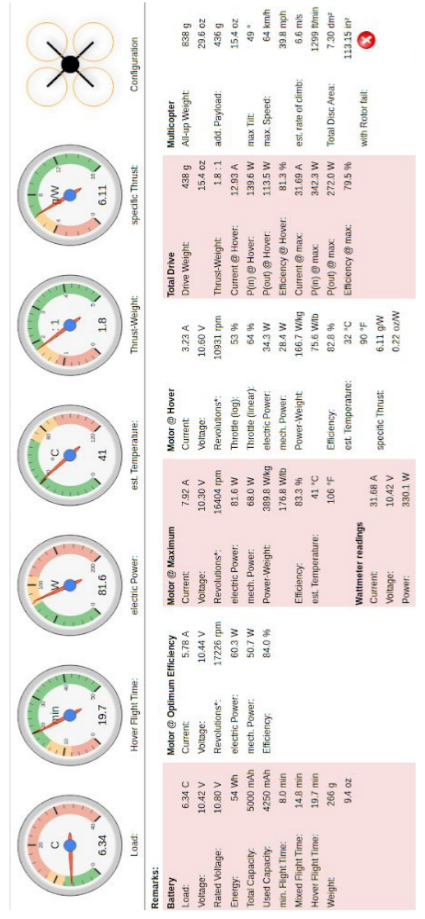
\includegraphics[height=\linewidth, angle=270]{image/ecalc.png}
    \caption{ECalc results for selected configuration}
    \label{fig:ecalc}
\end{figure}
Based on these parameters, a market research was carried out to find out the best possible configuration for the multirotor, which was the followed by testing on the online RC calculator ECalc as depicted in Fig \ref{fig:ecalc}.

\subsection{Battery Selection}
As the battery capacity increases so does its weight. Thus, flight time is not directly proportional to the battery capacity as depicted in \ref{fig:batcap}. Maximum current that can be drawn from any battery is equal to the battery capacity times the C- rating.
\begin{equation}
    Max\; Current = Battery\; Capacity * C\; rating
\end{equation}
Therefore, for the projected flight time of 18-25 minutes, a 5000mAh LiPo battery was selected.
\begin{figure}[h]
    \centering
    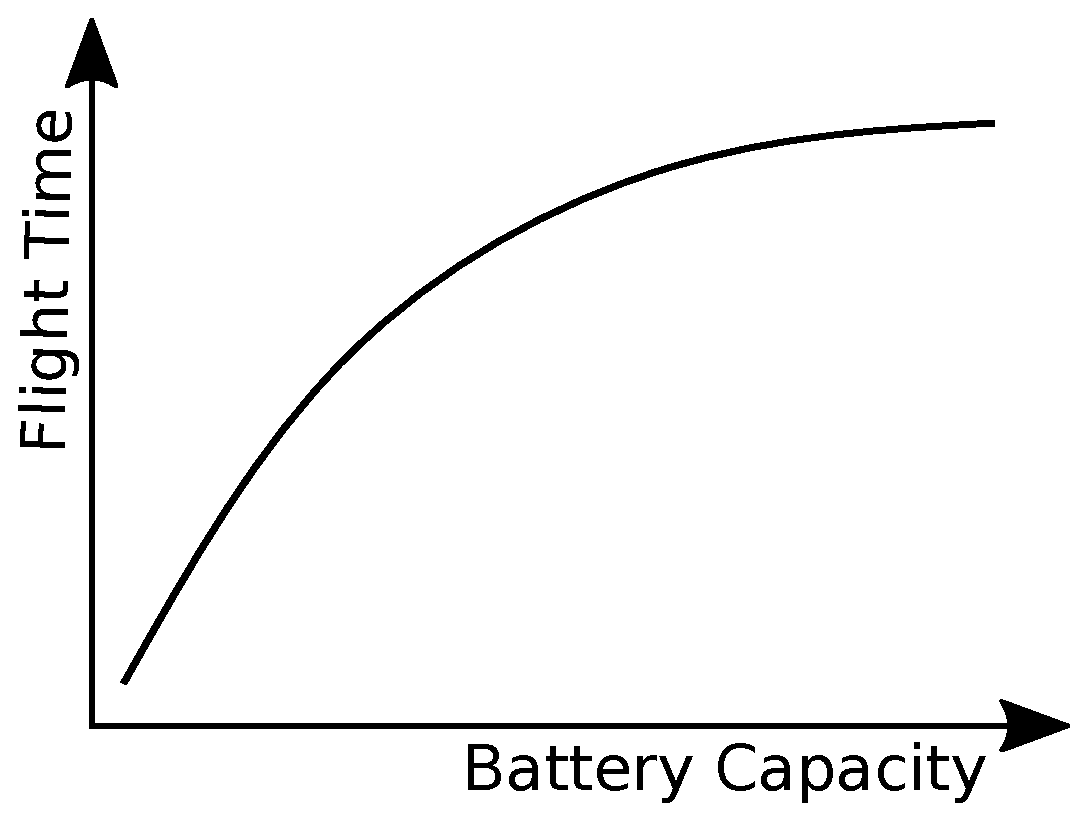
\includegraphics[width=0.7\linewidth]{image/batcap.eps}
    \caption{Flight Time vs Battery Capacity(mAh)}
    \label{fig:batcap}
\end{figure}

The final selected components for the quadrotor are tabulated in \ref{tab:selcomps} and the assembled prototype demonstrated in \ref{fig:proto}.

\begin{table}[h]
    \centering
    \caption{Selected Components}
    \begin{tabular}{c|c}
        \hline \textbf{Component} & \textbf{Product} \\\hline
        Frame & ZMR 450 mm \\
        Flight Controller & 3DR Pixhawk 2.4.8 \\
        Telemetry & Sik 433MHz Radio \\
        Motor & DJI 2212 920kv\\
        ESC & Afro 30Amp \\
        Radio Control & FlySky 2.4GHz RC \\
        Onboard Computer & Raspberry Pi 3B+ \\
        Intra-swarm & TPLink Wifi dongle \\
        Battery & Tattu 3300mAh 3S Lipo\\\hline
    \end{tabular}
    
    \label{tab:selcomps}
\end{table}

\begin{figure}[h]
    \centering
    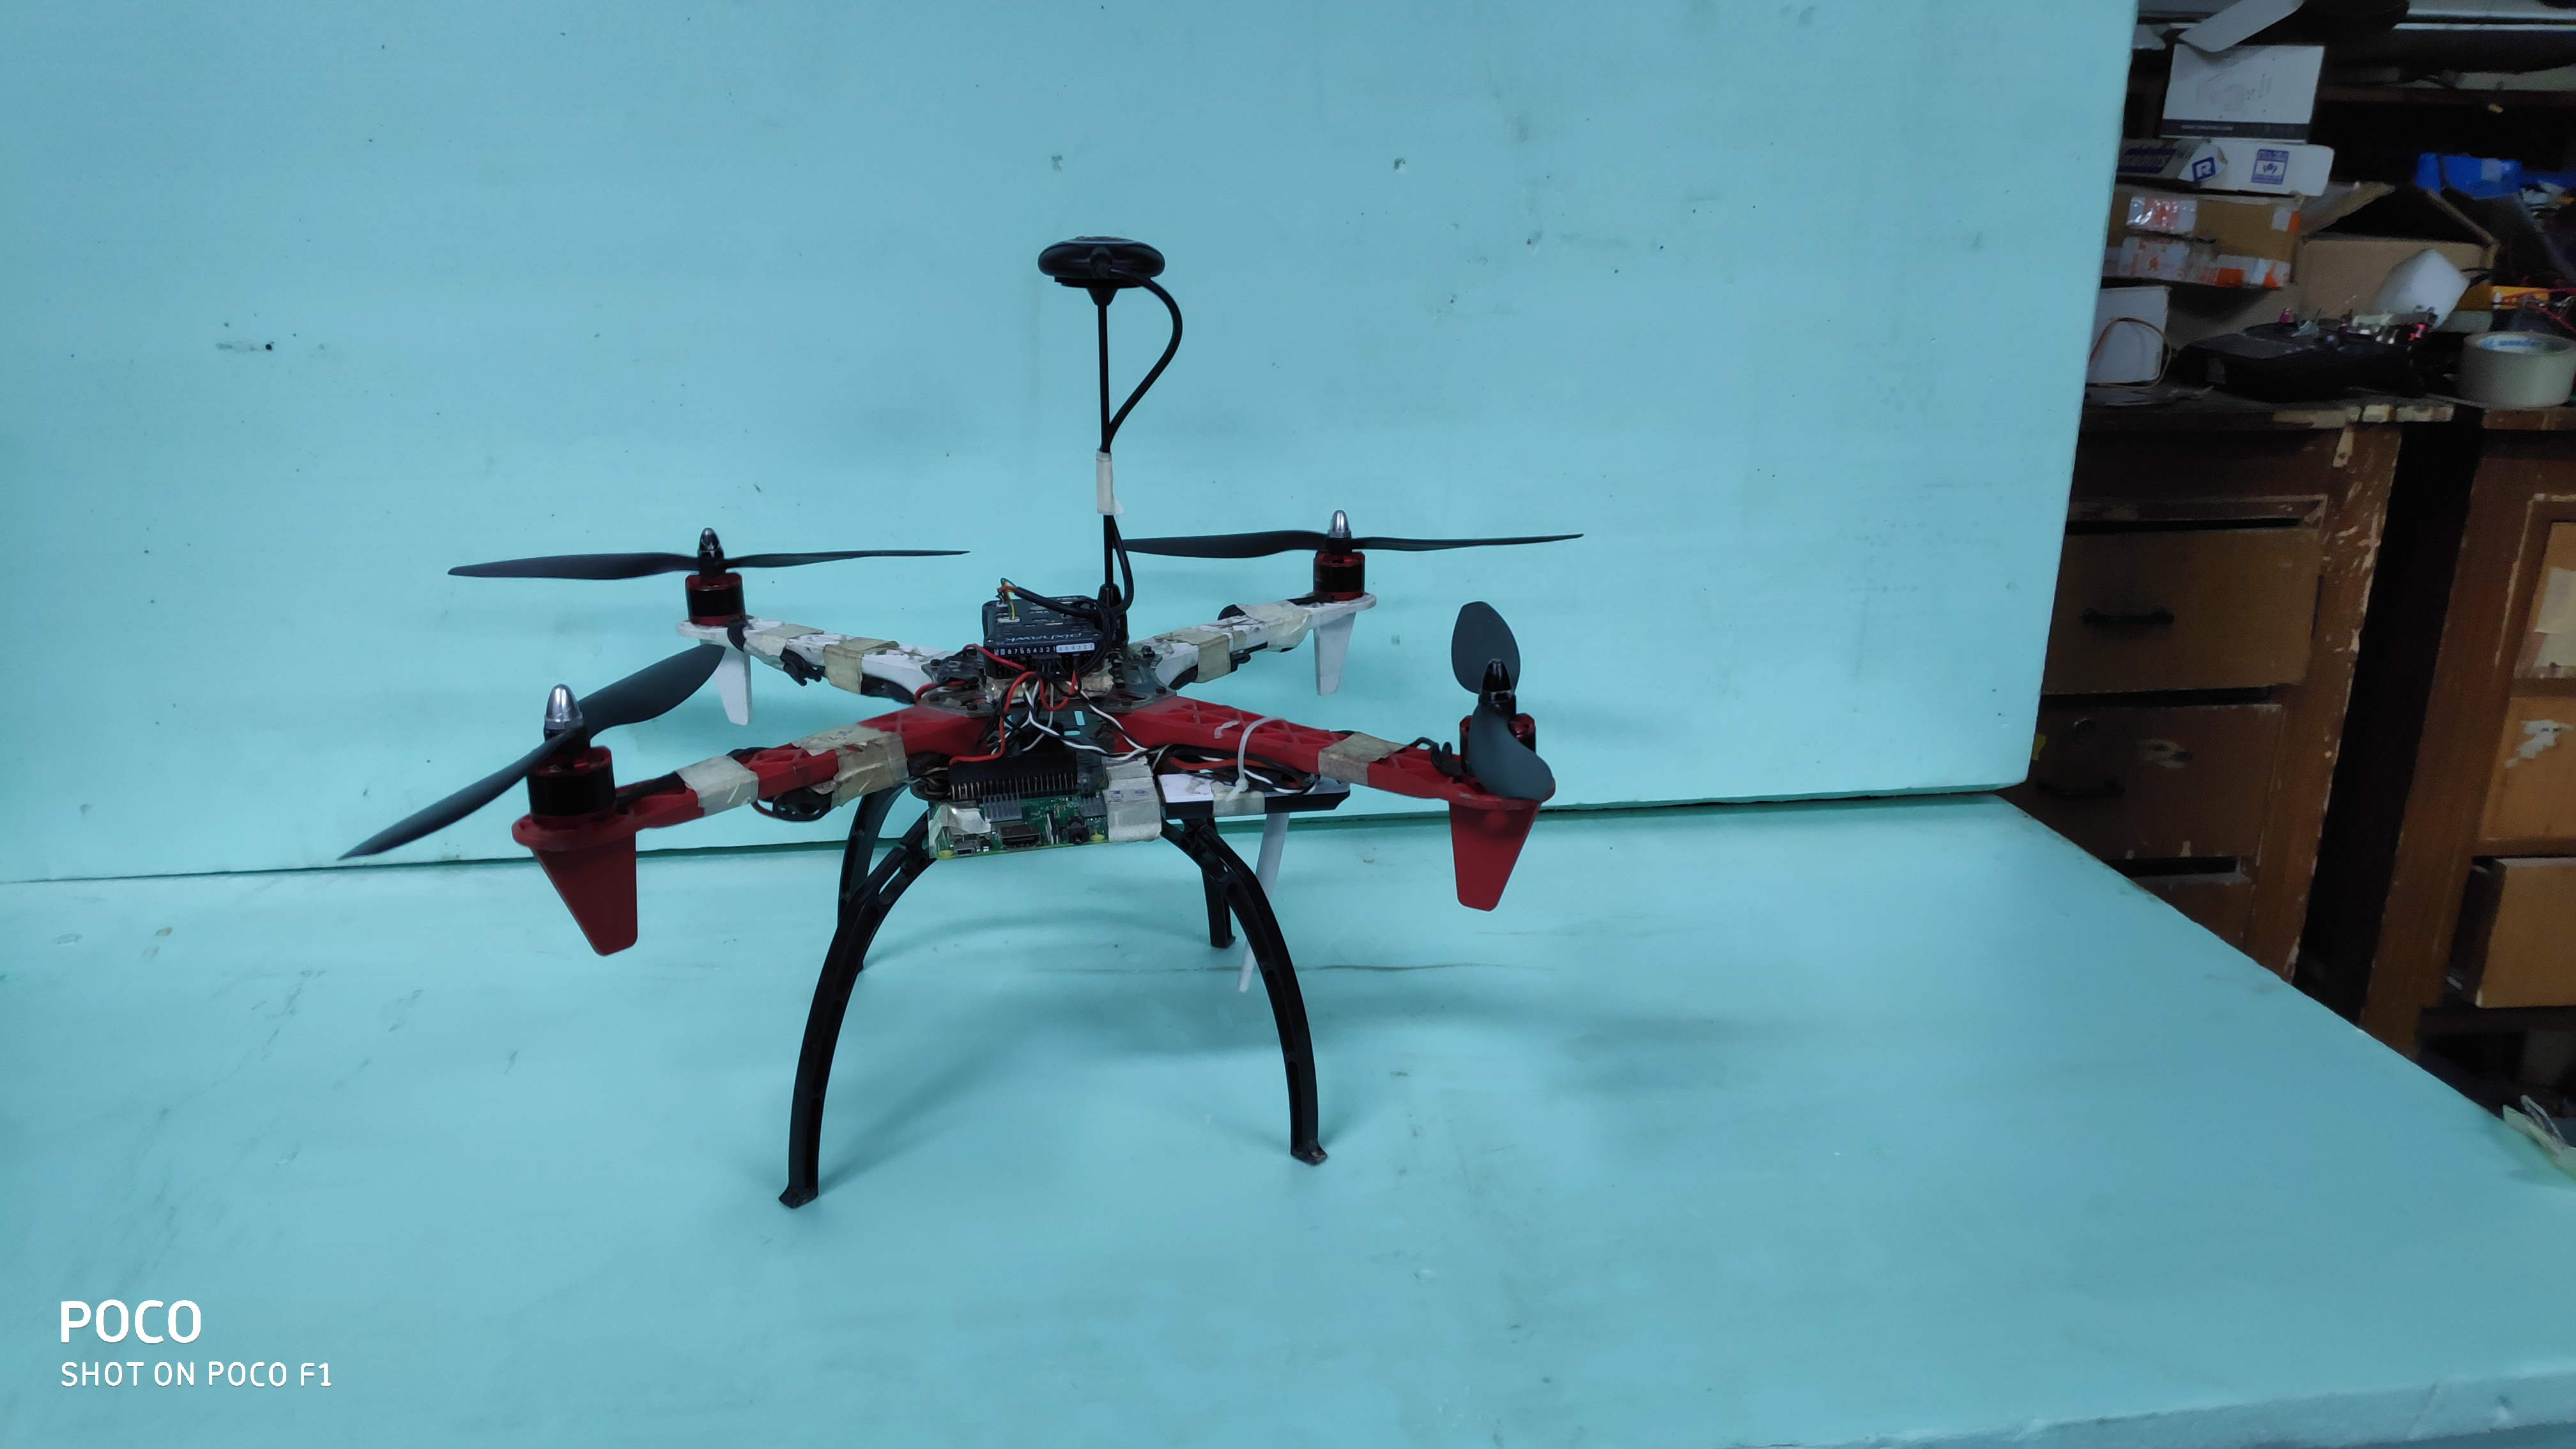
\includegraphics[width=0.8\linewidth, trim=350 200 1200 220,clip]{image/prototype.jpg}
    \caption{Prototype developed for testing}
    \label{fig:proto}
\end{figure}
\end{spacing}